% Parte I: O problema
% - Enunciado do PNCG; Hamiltoniana; integrais primeiras.
\begin{frame}[plain]
    \centering
    \vspace{0.5cm}
    \Huge Parte I: O Problema
\end{frame}

%------------------------------------------------

\begin{frame}
\justifying
\frametitle{PNCG}

O que é o problema de N-corpos gravitacional?

{\color{blue}\href{https://ime.usp.br/~oapotalej/arquivos/coloquinho2026/exemplos.html}{Vídeos dos exemplos.}}

\begin{columns}
    \column{.50\textwidth}\justifying
        \begin{figure}
            \centering
            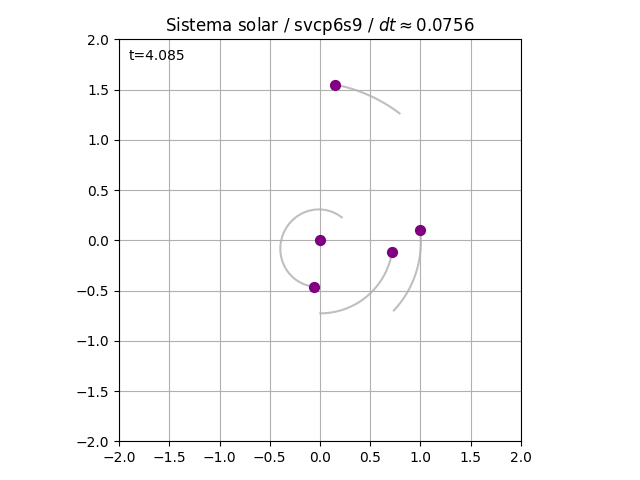
\includegraphics[width=\linewidth]{img/sistema_solar.png}
            \caption{Sistema solar}
        \end{figure}

    \column{.50\textwidth}\justifying
        \begin{figure}
            \centering
            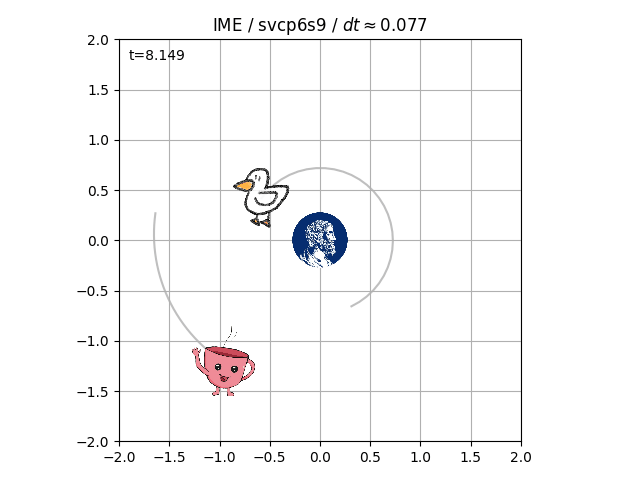
\includegraphics[width=\linewidth]{img/sistema_ime.png}
            \caption{Sistema IME}
        \end{figure}
\end{columns}

\end{frame}

%------------------------------------------------

\begin{frame}
\justifying
\frametitle{PNCG}

\begin{block}{Enunciado}
    O PNCG é um problema com $N$ partículas com massas $m_a$ e posições $\vet q_a$, regidas unicamente pelo potencial newtoniano:
    \begin{equation*}
        \ddvet q_a = \sum_{b \neq a} m_b \dfrac{\vet q_b - \vet q_a}{\norma{\vet q_b - \vet q_a}^3} = - \dfrac{1}{m_a} \derpar{V}{\vet q_a}, \quad a = 1, 2, ..., N.\footnote{Aqui omitimos a constante $G$ por facilidade, tomando $G=1$ e ignorando suas dimensões.}
    \end{equation*}
\end{block}
\pause
\begin{block}{Forma Hamiltoniana}
    Tomando o momento generalizado $\vet p_a$, podemos reescrever o problema via equações de Hamilton:
    \begin{equation*}
        \begin{cases}
            \dvet q_a = \partial H / \partial \vet p_a, \\
            \dvet p_a = - \partial H / \partial \vet q_a
        \end{cases},
        \quad H = \sum_{a=1}^N \dfrac{\norma{\vet p_a}^2}{2 m_a} + V(\vet q).
    \end{equation*}
\end{block}

\end{frame}

%------------------------------------------------

\begin{frame}
\justifying
\frametitle{PNCG: Integrais primeiras}

\begin{block}{Integrais primeiras}
    O PNCG (em 3 dimensões) tem 10 integrais primeiras.
    \begin{enumerate}
        \item Energia total $E \equiv H$;
        \item Momento angular total $\vet J = \sum_{a=1}^N \vet q_a \times \vet p_a$ (3 componentes);
        \item Momento linear total $\vet P = \sum_{a=1}^N \vet p_a$ (3 componentes);
        \item Movimento do centro de massas: $\vet G = M \vet q_{cm} - t \vet P$ (3 componentes).
    \end{enumerate}
\end{block}
\begin{block}{Centro de massas}
    O PNCG é invariante por translações, então tomamos sempre $\vet q_{cm}(t_0) = \vet 0$ sem perder generalidade.
\end{block}

\end{frame}

%------------------------------------------------
